\documentclass[12pt]{article}
\usepackage{amsmath,amssymb,amsthm,enumitem}
\usepackage{tikz-cd,xspace,graphicx,xcolor}
% \usepackage{amsmath,amssymb,amsthm,xspace,enumitem,xcolor}
% \usepackage{tikz-cd,xspace,graphicx,wrapfig,algorithm,lscape}
% \usepackage[noend]{algpseudocode}
% \usepackage[margin=1in]{geometry}
% \usepackage{etex,etoolbox}
\usepackage{wrapfig}
\usepackage[margin=1in]{geometry}

\newtheorem{theorem}{Theorem}
\newtheorem{lemma}{Lemma}
\newtheorem{corollary}{Corollary}
\newtheorem{definition}{Definition}

% !TeX root = main.tex

\newtheorem{theorem}{Theorem}
\newtheorem{lemma}{Lemma}
\newtheorem{corollary}{Corollary}
\newtheorem{definition}{Definition}

\newcommand{\R}{\mathbb{R}}
\newcommand{\N}{\mathcal{N}}
\renewcommand{\O}{\mathcal{O}}
\newcommand{\e}{\varepsilon}
\newcommand{\Pers}{\mathcal{P}}
\newcommand{\dist}{\mathbf{d}}
\newcommand{\dmax}{\dist_{\mathrm{max}}}
\newcommand{\Cech}{\v Cech\xspace}
\newcommand{\cech}{\check{\mathcal{C}}}
\newcommand{\rips}{\mathcal{R}}
\newcommand{\T}{\mathcal{T}}
\newcommand{\ball}{\mathbf{ball}}
\newcommand{\PPers}{\mathbb{P}}
\newcommand{\hf}{\hat{f}}
\renewcommand{\ker}{\mathbf{ker}\xspace}
\newcommand{\im}{\mathbf{im}\xspace}
\newcommand{\cok}{\mathbf{cok}\xspace}
\newcommand{\coim}{\mathbf{coim}\xspace}
\newcommand{\id}{\mathbf{1}}


\renewcommand{\restriction}{\mathord{\mid}}
\newcommand{\rest}{\mathord{\mid}}

\mathchardef\mhyphen="2D
\newcommand{\Z}{\mathbb{Z}}
\newcommand{\rad}{\mathrm{rad}}
\newcommand{\birth}{\mathrm{birth}}
\newcommand{\death}{\mathrm{death}}
\newcommand{\pers}{\mathrm{Pers}}
\newcommand{\bary}{\mathrm{Bary}}
\newcommand{\kbary}{k\mhyphen\mathrm{Bary}}
\newcommand{\kcover}{k\mhyphen\mathrm{Cover}}
\newcommand{\cent}{\mathrm{center}}
\newcommand{\JL}{\textsc{JL}\xspace}
\newcommand{\conv}{\mathrm{conv}}
\newcommand{\power}{\mathcal{P}}
\newcommand{\C}{\mathcal{C}}
\newcommand{\nrv}{\text{Nerve}}
\newcommand{\Hom}{\mathrm{Hom}}
\newcommand{\knrv}{k\mhyphen\mathrm{Nerve}}
\newcommand{\clique}{\mathrm{Clq}}
\newcommand{\F}{\mathcal{F}}
\newcommand{\G}{\mathcal{G}}
\newcommand{\Rips}{\mathrm{Rips}}
\newcommand{\projectionOf}[1]{\overline{#1}}
\newcommand{\Pbar}{\projectionOf{P}}
\newcommand{\Sbar}{\projectionOf{S}}
\newcommand{\Tbar}{\projectionOf{T}}
\DeclareMathOperator*{\argmin}{argmin}
\newcommand{\wfs}{\mathrm{wfs}}
\newcommand{\reach}{\mathrm{reach}}
\newcommand{\hocolim}{\mathrm{hocolim}\;}
\newcommand{\dgm}{\mathrm{dgm}\xspace}

\renewcommand{\because}[1]{& \left[\text{#1}\right]}

\newcommand{\D}{{\mathcal{D}}}
% \newcommand{\B}{{\mathcal{B}}}
\renewcommand{\O}{\mathcal{O}}
\newcommand{\I}{{\mathcal{I}}}
\newcommand{\K}{{\mathcal{K}}}
% \newcommand{\U}{{\mathcal{U}}}
% \newcommand{\V}{{\mathcal{V}}}
\newcommand{\start}[1]{\noindent {\bf #1}\hspace{2ex} }
\newcommand{\mcal}[1]{\mathcal{#1}}
\newcommand{\mbb}[1]{\mathbb{#1}}
\newcommand{\ind}{\hspace{3ex}}
\newcommand{\collar}{(\overline{\mathcal{D}\setminus\mathcal{B}})}
\renewcommand{\hom}{\mathrm{H}}
% \renewcommand{\hom}{\mathbf{H}}
\newcommand{\rco}{\tilde{\hom}}
\newcommand{\rank}{\mathbf{rk\xspace}}
\newcommand{\rk}{\mathbf{rk\xspace}}
\newcommand{\comp}[1]{\overline{#1}}
\newcommand{\jung}{\vartheta}
\newcommand{\jungd}{\jung_d}
\newcommand{\norm}[1]{\|#1\|}
\newcommand{\cov}{\mathrm{cov}}
\newcommand{\U}{\mathbb{U}}
\newcommand{\V}{\mathbb{V}}
\newcommand{\W}{\mathbb{W}}
\renewcommand{\H}{\mathbb{H}}
\newcommand{\cl}{\mathbf{cl\xspace}}
\newcommand{\intr}{\mathbf{int\xspace}}
%\newcommand{\bary}{\text{bary}~}
\renewcommand{\dim}{\mathbf{dim}\xspace}

% \renewcommand{\b}{B_{\omega-c(\gamma - \delta)}}
% \newcommand{\bb}{\b^{\gamma - \delta}}
% \newcommand{\B}{B_\omega}
% \newcommand{\BB}{B_{\omega + c(\gamma + \delta)}}
%
% \newcommand{\Q}{Q_{\omega - c\delta}}
% \newcommand{\QQ}{Q_{\omega + c\gamma}}


\newcommand{\of}{{\delta}}
\newcommand{\off}{{2\delta}} % {{\gamma - \delta}} %
\newcommand{\offf}{{\gamma}} % {{3\delta}}

\newcommand{\ome}{\omega}
\renewcommand{\o}{\ome - c(\delta+\zeta)} % {\ome - c(\off)} % {\ome - 2c\of}
\newcommand{\oo}{\ome + c(\delta+\zeta)} % {\ome + 4c\of}

\renewcommand{\b}{B_{\o}}
\newcommand{\bb}{B_\omega}%{\b^{\offf - \of}} % {\b^{\off}} %
\newcommand{\B}{B_{\ome}}
% \newcommand{\BB}{B_{\oo}}

\newcommand{\fen}{\ome - c\zeta}
\newcommand{\fenn}{\ome + c\of}

\newcommand{\Q}{Q_{\fen}}
\newcommand{\QQ}{Q_{\fenn}}

% \renewcommand{\P}{P^{\of}}

\newcommand{\cmp}[1]{\overline{#1}}

\newcommand{\X}{\mathbb{X}}
\newcommand{\Y}{\mathbb{Y}}

\newcommand{\FQ}{\mathcal{Q}}
\newcommand{\FP}{\mathcal{P}}
\newcommand{\FB}{\mathcal{B}}

% \newcommand{\subi}[1]{_{{\scriptstyle (#1]}}}
% \newcommand{\subi}[1]{_{\scalebox{1}{$\scriptscriptstyle (#1]$}}}
\newcommand{\subi}[1]{_{\scriptscriptstyle (#1]}}
% \newcommand{\P}[1]{P_{{\scriptstyle (#1]}}}

% \newcommand{\A}{\mathbb{A}}
% \newcommand{\BE}{\mathbb{B}}
\renewcommand{\S}{\mathbb{S}}
\renewcommand{\T}{\mathbb{T}}
\renewcommand{\U}{\mathbb{U}}
\renewcommand{\V}{\mathbb{V}}
\renewcommand{\W}{\mathbb{W}}

\renewcommand{\D}[2]{\mathcal{D}_{#1}[#2]}
\newcommand{\DD}[1]{\mathbb{D}_{#1}}


\newcommand{\E}{\mathcal{E}}
\renewcommand{\P}[3]{\mathcal{P}_{#1}^{#2}[#3]}
\newcommand{\CP}[3]{\cech\mathcal{P}_{#1}^{#2}[#3]}
\newcommand{\RP}[3]{\rips\mathcal{P}_{#1}^{#2}[#3]}

\newcommand{\PP}[2]{\mathbb{P}_{#1}^{#2}}
\newcommand{\CPP}[2]{\cech\mathbb{P}_{#1}^{#2}}
\newcommand{\RPP}[2]{\rips\mathbb{P}_{#1}^{#2}}

\renewcommand{\AA}{\mathbb{A}}
\newcommand{\BB}{\mathbb{B}}

% \newcommand{\ext}[1]{\widehat{#1}}
\newcommand{\ext}[1]{\E\xspace #1}
\renewcommand{\I}{\mathcal{I}}
\newcommand{\J}{\mathcal{J}}


\newcommand{\cU}{\mathcal{U}}
\newcommand{\cV}{\mathcal{V}}
\newcommand{\cF}{\mathcal{V}}
\newcommand{\A}{\mathcal{A}}
\newcommand{\FF}{\mathbb{F}}


\title{From Coverage Testing to Topological Scalar Field Analysis}
\author{Kirk P. Gardner}

\begin{document}

\maketitle

% !TeX root = ../main.tex

\begin{abstract}
  The topological coverage criterion (TCC) can be used to test whether an underlying space is sufficiently well covered by a given data set.
  Given a sufficiently dense sample, topological scalar field analysis (SFA) can give a summary of the shape of a real-valued function on its domain.
  The goal of this paper is to put these theories together so that one can test coverage with the TCC while computing a summary with SFA.
  The challenge is that the TCC requires a well-defined boundary that is not generally available in the setting of SFA.
  To overcome this, we show how the scalar field itself can be used to define a boundary that can be used to confirm coverage.
  % This requires a generalization of the TCC proof and resolves one of the major barriers to wider use of the TCC.
  This requires an interpretation of the TCC that resolves one of the major barriers to wider use.
  % It also extends SFA methods to a wider class of spaces.
  It also extends SFA methods to the setting in which coverage is only confirmed in a subset of the domain. %a space surrounded by a sub-levelset.
  % We show how the intersection of these two theories can be used to approximate the persistent homology relative to a static sublevel set.
  % We then discuss how this persistent relative homology relates to that of the scalar field as a whole.
\end{abstract}


\section{Introduction}
% !TeX root = ../main.tex

Data can often be viewed as a sample of a function on some unknown space.
Determining if this sample sufficiently \emph{covers} the underlying space is a fundamental question for any meaningful analysis.
Taking the sample as points in some unknown metric space, coverage requires that the underlying space is contained in the union of metric balls centered at points in the sample.
The radius of these metric balls determines the scale at which the space is covered.
Often, data is provided without coordinates, and only pairwise connectivity information that indicates when sample points are within some fixed distance.
Testing for coverage in this setting is a problem that is essentially topological in nature.
Homology is a tool from algebraic topology that can be used to compute coverage holes from pairwise connectivity information alone.
% That is, given only pairwise connectivity information, homology can detect the holes in a cover that may indicate a lapse in coverage.
However, holes in a cover may not indicate a lack of coverage, as these holes may be properties of the underlying space.
Moreover, not all lapses in coverage appear as holes in the cover, as there may be regions of the space that have not bee sampled at all.
Verifying coverage therefore requires information about the boundary of the space that is captured by its homology.

The Topological Coverage Criterion (TCC) is a computable condition for coverage that uses homology along with topological priors in a coordinate-free setting.
That is, given only pairwise connectivity information, the TCC uses information about the boundary of a space to confirm coverage using relative homology.
In its original form this required that the sample points near the boundary were labelled manually---without coordinates, there is no way to determine these points analytically.
This requirement is perhaps the main reason why the TCC can so rarely be applied in practice.
For points sampled from a real-valued function, it can be shown that this requirement can be replaced with assumptions about the function itself.
One can then use prior information about the homology of the function above (or below) a given scalar value to confirm coverage of a \emph{part} of the domain.

While data coverage is an important property throughout data analysis, it has an important role to play in topological approaches to data.
These techniques provide novel information about the structure of data, and coverage provides a way to attribute that structure to the underlying space.
In particular, \emph{persistent homology} decomposes the homology of a space by a sequence of subspaces to produce a robust topological signature known as a persistence \emph{barcode} or \emph{diagram}.
For a real-valued function this sequence is defined by its sub or super level sets.
The resulting signature is invariant to continuous transformations, and is therefore a useful signature for use with non-deterministic statistical techniques.
Topological Scalar Field Analysis (SFA) approximates the persistent homology of a real-valued function from a finite sample.
The fundamental assumption made in SFA is that this sample covers the domain at some scale, and the quality of the approximation is proportional to this scale.

Given a finite sample of a real-valued function both the TCC and SFA apply homology in a coordinate-free setting.
By modifying the statement of the TCC information about the persistent homology of the function can be used as topological priors.
In fact, it can be shown that the TCC can be extracted from the persistent relative homology of a sample.
One can then verify the quality of an approximation directly from a variation of the signature computed in SFA.
In addition, careful observations about the TCC itself indicate that

% Moreover, this variation supports instances of partial coverage
The proposed work will unify the TCC and SFA as a way to provide verified scalar field analysis.
This first requires adapting the TCC to bounding subsets of the domain defined by the function itself.
It also requires a new stability proof for approximating the persistent homology of a real-valued function modulo a static.
In addition to providing a theoretical framework for the unification of these two theories, this work will explore the significance of the resulting relative persistent homology.

A key observation in this work is that the TCC confirms not only coverage, but that the sample is \emph{topologically representative} of the domain for a given range of function values.
Using this observation, a number of connections with existing work on Extended persistence and level set persistence will be explored.
In particular, the TCC can be viewed as confirming the presence of a \emph{fundamental class} that can be used to compute \emph{topological duals}.
Additional work is motivated by an application involving Lipschitz extensions that requires computing these topological duals within the persistence computation.
This will extend the existing theory of persistent (co)homology to support duality via the cap product with a fundamental class.

% Specifically, the objectives of this work are as follows:
%
% \begin{itemize}
%   \item A theorem for verified SFA that unifies the assumptions made by the TCC and those required by SFA.
%   \item An efficient algorithm for merging the relative persistence diagrams produced.
%   \item An investigation of how SFA can be used
% \end{itemize}
%
% the persistence diagram of the function
% One of the main goals is to provide a theorem for verified SFA that unifies the assumptions made by the TCC and those required by SFA


\section{Background}
% !TeX root = ../main.tex

% This body of work comprises much of the relevant theoretical foundations for persistent homology for data analysis in general.
We refer to the following process as \emph{topological scalar field analysis (SFA)}.
The goal is to approximate the persistent homology of a real valued function $f : D\to \R$.
The input is a sample of the function that covers its domain the domain at some scale $\delta > 0$.
A nested pair of simplicial complexes that captures the homology of the cover is then constructed on these points.
These complexes are sorted by the function values on its vertices to form a sequence of nested sub complexes known as a \emph{filtration}.
The standard reduction algorithm~\cite{edelsbrunner02simplification,zomorodian05computing} is then used to compute its persistent homology.
Stability results state that, because the vertices cover the domain at scale $\delta$, the corresponding persistence barcode is a $\delta$-approximation to that of the function itself~\cite{cohensteiner07stability,chazal09proximity}.

The primary assumption in SFA is that the sample covers the domain at some scale $\delta$.
The Peristent Nerve Theorem~\cite{chazal08towards} can then be used to show that the nested pair of simplicial captures the homology of the cover.
These nested pairs, which will be viewed as images of a map induced by inclusion, will be referred to as \emph{short filtrations}.

For a bounded $d$-dimensional domain the TCC uses the fact that the number of generators in the top-dimensional relative homology of the domain modulo its boundary is equal to the number of connected components~\cite{desilva07coverage}.
Given a finite sample $P$ and a sub-sample $Q\subseteq P$ of points near the boundary one can therefore check that the sample covers the domain at scale $\delta > 0$ by comparing number of generators in the top-dimensional relative homology of the pair $(P^\delta, Q^\delta)$ to the number of connected components of the domain.
A key observation is that this test not only confirms that the sample covers the domain, but also that we have a sub-sample of points $Q^\delta$ that resembles its boundary.
We refer to this property as being \emph{topologically representative} of the domain and its boundary.

In its original form the TCC is stated as a criteria for coverage by a sensor network in a coordinate free setting---coordinates of sensors are not provided, only some limited connectivity information.
The input is a pair of neighborhood graphs on $P$ that can be used to construct a short filtration of (Vietoris-)Rips complexes that captures the homology of the cover $(P^\delta, Q^\delta)$.
However, because there is no way to determine which points are close to the boundary analytically the TCC requires that these points $Q$ are labeled manually.
This requirement is perhaps the main reason why the TCC can so rarely be applied in practice.
It can be shown that this requirement can be removed by instead requiring that our input points sample some unknown $c$-Lipschitz function $f : D\to \R$.
This is more natural for applications to data analysis, where data represents local measurements of some underlying process.
Given a threshold $\omega\in\R$ such that the $\omega$-sub levelset $f^{-1}((-\infty,\omega])$ contains the boundary we can instead define $Q$ by function value.
The existence of this threshold, as well as additional \emph{regularity assumptions}, can then be phrased in terms of the persistent homology of the function.

% This requirement is natural for applications to data analysis, where data represents local measurements of some underlying process.
% Given a threshold on function values that can be used to define a bounding subset of the domain we can define our sampled boundary by their function values alone.
% The existence of this threshold, as well as additional \emph{regularity assumptions} that are required in order to establish the minimum resolution of the sample, can then be phrased in terms of the persistent homology of the function.
% % Moreover, the TCC requires additional \emph{regularity assumptions} that are required in order to establish the minimum resolution of the sample.
% % Traditionally, these assumptions required information about the geometry of the domain, and were made in terms of the \emph{smoothness} of its boundary.
% % Now, these assumptions can be stated directly in terms of the persistent homology of the function itself.

% Now, the TCC requires information about the persistent homology of the function.
From this perspective, information about the persistent homology of a function is required in order to confirm coverage.
Conversely, approximating the persistent homology of a function requires coverage.
In fact, the persistence computation and the TCC overlap in a number of ways.
The coverage condition can therefore be extracted directly from the approximated diagram persistence diagram, and the quality of the approximation depends on coverage.
Not only is the criterion encoded in this diagram, but its computation produces a \emph{fundamental class} for the domain that can be used to compute topological duals.
It is in this way that one can verify that a persistence diagram is representative of the scalar field by leveraging topological priors similar to those required by the TCC.
Moreover, the use of relative homology and duality in the TCC can be used to extend SFA to the setting of \emph{partial coverage}.


\section{Related Work}
% % !TeX root = ../main.tex

TDA is concerned with the ``shape of data,'' and has found applications in
neuroscience~\cite{saggar2018towards, sizemore2019importance},
structural biology~\cite{gameiro2015topological,kovacev2016using,dey2018protein},
medical imaging~\cite{carlsson2008local,robins2011theory,bendich2016persistent},
geometry processing~\cite{skraba2010persistence,poulenard2018topological,bruel2020topology},
and machine learning~\cite{clough2019explicit,chen2019topological,carlsson2020topological,gabrielsson2020topology}, to name a few.
A number of approaches can be considered topological in nature, and \textbf{todo}.
Among these are \textbf{todo}.
However, much of the theoretical work over the last decade has been focused on \emph{persistent homology}.

Persistent homology was first introduced by Edelsbrunner, Letscher, and Zomorodian in 2002~\cite{edelsbrunner02simplification}.
This work introduced the standard \emph{reduction algorithm} for computing the persistent homology of simplicial complexes in $\R^3$ with $\Z_2$ coefficients.
The output is a \emph{persistence diagram} or \emph{barcode} that encodes the ``birth'' and ``death'' of homological features of the complex.
Later work by Zomorodian and Carlsson provided a more general form of the reduction algortithm for filtered spaces with coefficients in a field~\cite{zomorodian05computing}.
This work also introduced the notion of an \emph{persistence modules} and persistence barcodes as \emph{interval decompositions} of these modules.
\textbf{First instance of the structure theorem?}
This set the stage for a series of work that established stability results for general persistence modules.

\paragraph{Theoretical Foundations}

Initial stability results by Cohen-Steiner, Edelesbrunner, and Harer were proved for the persistent homology of real-valued functions~\cite{cohensteiner07stability}.
This work was later extended to persistence modules in general by Chazal et al. which introduced the notion of a \emph{$\delta$-interleaving} of persistence modules~\cite{chazal09proximity}.
Their main result was the \emph{algebraic stability theorem}, which roughly states that the existence of a $\delta$-interleaving indicates a $\delta$-matching between their persistence barcodes.
Later work on the \emph{isometry theorem} showed that the converse is also true~\cite{todo}.
Importantly, the isometry theorem established the relationship between interleavings of persistence and the \emph{bottleneck distance} between their barcodes, providing a computable metric on the space of persistence diagrams that is stable with respect to the Gromov-Hausdorff distance between spaces.

Additional work has been done on persistence modules in general including multidimensional persistence, categorical interpretations, \textbf{todo}.
For persistent homology, this robust foundation allowed researchers to establish important inference and approximation results in the more general language of persistence modules.
Among these is relevant work by Chazal et al. that proved stability results for the persistent homology of scalar-valued functions approximated by Vietoris-Rips complexes~\cite{chazal09analysis}.
This work showed that, given a sample $P$ of a scalar valued function that \emph{covers} the domain of the function at scale $\delta$, the persistent homology of a nested sequence of Rips complexes filtered by function values on its vertices is $\delta$-interleaved with that of the scalar field itself.
Later work applied this theory to approximate the persistent homology of probability density function~\cite{chazal2013persistence}.

\paragraph{Stability and TDA}

This body of work comprises much of the relevant theoretical foundations for persistent homology for data analysis in general.
In particular, we refer to the following process as \emph{topological scalar field analysis (SFA)}.
The input is a simplicial complex that represents a discretization of some unknown domain.
The simplicial complex is then \emph{filtered} by a scalar valued function on its vertices, representing some underlying process on the domain.
The standard reduction algorithm~\cite{edelsbrunner02simplification,zomorodian05computing} can then be used to compute the persistent homology of this filtered simplicial complex.
Stability of results state that, provided an interleaving of the persistence module computed in theory, the corresponding persistence barcode is an approximation of that of the function itself~\cite{cohensteiner07stability,chazal09proximity}.

% It is in this way that the general theory of persistence modules provides
%
% \textbf{Question:} What algebraic tools can we use to analyze persistent \emph{homology} modules that we cannot use for persistence modules in general?
% \textbf{Exact sequences, relative homology, duality, etc}.
% \textbf{Pair groups?}
%
% An important step in this process is computing the persistent homology of a homological image.
% While this computation is straightforward for trivial maps such as those induced by inclusion\textbf{todo}.
% Cohen-Steiner, Edelsbrunner, Harer, and Morozov provide a theoretical analysis and algorithm for computing images, kernels, and cokernels of maps between persistence diagrams.
% \textbf{todo...}




\paragraph{Algorithms and Cohomology}

Many of these steps have since been improved, and a number of useful tools from algebraic topology have been leveraged to offer different perspectives on persistent homology in general.
% Rips complexes can be sparsified~\cite{todo} or replaced with other complexes\textbf{todo}
Importantly, the original reduction algorithm has been improved in a number of ways, including \textbf{todo distibuted, parallel, row/column operations, chunking, twisting, bopping}.

A key observation in computing persistent homology efficiently is to compute \emph{persistent cohomology}.
As vector spaces, cohomology is dual to homology, and for reasonable spaces it is known that the persistence barcodes produced by persistent homology and cohomology are the same~\cite{todo}.
This allows one to compute persistent cohomology instead of persistent homology, and this is often more efficient.
In fact, the reduction algorithm is shown to be the same for persistent homology an cohomology, simply acting in opposite directions~\cite{desilva11duality}.
However, while the barcodes produced are the same, the information captured by homology and cohomology is not.
While homology operates on \emph{cycles} representing \emph{holes} cohomology operates on \emph{cocycles} representing \emph{obstructions}.
Each feature of a barcode is associated with a representative (co)cycle that is often considered a by-product of the persistence computation.
In fact, many recent modifications to the reduction algorithm explicitly abandon these representatives for efficiency~\cite{todo}.
However, these representative encode useful information, and some interesting applications specifically require cocycle representatives~\cite{desilva11circular}.

\paragraph{Homological Sensor Networks and Short Filtrations}

The application of homology to coordinate-free sensor networks is a novel application of homology in that it is minimally persistent.
De Silva and Ghrist first introduced homological sensor networks (HSNs) as a collection of problems that applied homology to the problem of coverage testing without coordinates~~\cite{desilva06coordinate,desilva07homological}.
The underlying idea requires no persistence, and simply observes that, for a bounded $d$-dimensional space, the $d-1$ dimensional homology of a cover contains the information needed to confirm coverage.
Provided a sub-cover of the boundary this information is captured in the $d$ dimensional relative homology of the cover modulo the sampled boundary.
Work on HSNs culminated in the Topological Coverage Criterion~\cite{desilva07coverage} which computes this relative homology using a nested pair of (Vietoris-)Rips complexes.
The nested pair is factored through the \v Cech complex which is known to be homotopy equivalent to the cover by the Nerve Theorem~\cite{hatcher01}.
There has been a great deal of additional work on homological sensor networks including mobile networks and evasion paths, \textbf{todo}.
However, we will focus on this foundation, and how the use of relative homology and the Rips-\v Cech factoring process, which we refer to as an example of a \emph{short filtration}, relates to SFA and the broader theory of persistent homology.

While the use of short filtrations can be considered persistent homology their purpose is generally as a de-noising technique.
Taken instead as the image of homomorphisms between persistence modules, themselves persistence modules, short filtrations can be used with persistence without the need for multidimensional persistence~\cite{todo}.
A canonical example that motivates the proposed work is the use of short filtrations in SFA.
In SFA, the Persistent Nerve Theorem~\cite{chazal08towards} is used with a nested sequences of Rips complexes to prove stability results in a similar way.

As a note, the images, kernels, and cokernels of maps in homology are particularly useful due to their use in \emph{exact sequences}.
Cohen-Steiner, Edelsbrunner, Harer, and Morozov extend persistent homology to images, as well as kernels and cokernels, of persistence modules, and provide an algorithm for computing them in general~\cite{cohen09persistent}.
Much of the proposed work is inspired by the use of relative homology in the TCC and how persistence module homomorphisms can be interpreted in terms of the long exact (co)homology sequences of pairs and triples.

% In this sense SFA can be thought of as an extension of the TCC to \emph{persistent} homology, and their inputs and outputs are in some sense dual.


% \paragraph{Persistence and Homological Algebra}
%
% Duality is just one example of a tool from algebraic topology that can be used not only as a method of proof, but also for creating efficient algorithms.
% These tools can be exploited using the framework provided by the general theory of persistence modules in the special case of persistent (co)homology.
% For example, a standard approach in the analysis of point cloud data is to factor a nested pair of Rips complexes through the \v Cech which, by the Persistent Nerve Theorem~\cite{chazal08towards, todo}, captures the persistent homology of the associated cover.
% Using the fact that the image of a map between persistence modules is a persistence module
%
%
% While implementing this Cohen-Steiner, Edelsbrunner, Harer, and Morozov

\paragraph{Duality and Coverage}

% \begin{itemize}
%   \item Other work on duality in persistent homology
%   \item Other work in homological sensor networks
%   \item Duality, complements of spaces, and relative persistence
%   \item Relationship to scalar fields and level sets
%   \item Extended persistence (and local homology?)
% \end{itemize}

The duality between homology and (co)homology is a powerful tool that has seen limited use in modern persistence.
Much of the theory of algebraic topology developed in the late 20th century focused on this duality for general spaces~\cite{spanier66algebraic,munkres84elements,bredon93,hatcher01}.
Poincar\'e duality states that the cap product with fundamental class provides a natural isomorphism between the $k$th cohomology and the $d-k$th homology of a closed, orientable $d$-manifold.
There are a number of variants to Poincar\'e duality such as Lefschetz duality for manifolds with boundary, and Alexander duality for compact subspaces of the sphere.

Perhaps the first application of duality in TDA was the use of Alexander duality in the TCC.
Here, Alexander duality relates the top-dimensional relative homology of a space modulo its boundary to the zero dimensional homology of its complement.
This greatly simplified their analysis by allowing them to reason about zero dimensional homology instead of connectedness in arbitrary dimension.
Similarly, in SFA, duality can be used to relate the persistent homology and cohomology of sub and super levelset filtrations of a real-valued function.
This fact is used  in work by Cohen-Steiner, Edelsbrunner, and Harer on Extended Persistence~\cite{cohen09extending} in which Poincar\'e and Lefschetz duality are used explicitly to construct an extended persistence diagram.
% In extended persistence an extended filtration first ascends with the $k$ dimensional homology of the sub levelset filtration, ending with the $k$ dimensional homology of the manifold.
% By Poincar\'e duality the $k$ dimensional homology of a $d$-manifold is isomorphic to its the $d-k$ dimensional cohomology.
% Because cohomology is contravariant, the sequence can then be extended to a \emph{descending} sequence of sub level sets.
% Taking each sub and super levelset as a submanifold with boundary Lefschetz duality and excision can be used to replace $d-k$ dimensional cohomology with $k$ dimension relative homology of the manifold modulo the corresponding \emph{super} level set.
% It is in this way that extended persistence provides an excellent example of how duality can be used to unify the persistent homology of sub level sets and the relative persistent homology of super level sets.
% Later work made this connection explicit, by formally establishing the dualities between both absolute and relative variants of homology and cohomology.
In both of these cases the existence of an isomorphism provided by duality is sufficient.
Little work has been done to apply duality in persistent homology as a general tool in TDA.
% The construction of the isomorphism between homology and cohomology in Poincar\'e duality is provided by the cap product with a \emph{fundamental class}.
% Similarly, the relative variations of Lefschetz, and complements of spaces in Alexander duality can be stated in terms of relative cap products.

% However, in this and many other cases duality is used only as a method of proof.
% % This allows their proof to be greatly simplified by reasoning about zero dimensional homology, connectedness, instead of connectedness in arbitrary dimension.
% % Later work attempted to make this approach more explicit, and integrated\textbf{todo}~\cite{cavanna2017when}.
% % While this is an interesting example of how duality can be applied as a method of proof, the use of Alexander Duality in this case is lacking.
% % In fact, much of the work on duality in persistent homology lacks rigor
% % A fascinating subset of algebraic topology in general works towards general duality theorems that establish the relationship between
% %
% % The TCC has been expanded in a number of directions including \textbf{TODO}.
% % In particular, a great deal of work on the problem of evasion paths, which \textbf{TODO}.
% % \textbf{TODO how is duality used here}.
% % \textbf{Zigzag homology, parameterized homology, Alexander duality for parameterized homology.}

% !TeX root = ../main.tex

Topological Data Analysis (TDA) is an emerging field that is concerned with the ``shape of data,'' and has found applications in
neuroscience~\cite{saggar2018towards, sizemore2019importance},
structural biology~\cite{gameiro2015topological,kovacev2016using,dey2018protein},
medical imaging~\cite{carlsson2008local,robins2011theory,bendich2016persistent},
geometry processing~\cite{skraba2010persistence,poulenard2018topological,bruel2020topology},
and machine learning~\cite{clough2019explicit,chen2019topological,carlsson2020topological,gabrielsson2020topology}, to name a few.
A number of approaches can be considered topological in nature, and \textbf{todo}.
Among these are \textbf{todo morse theory, sheaves, ...}.
However, much of the theoretical work over the last decade has been focused on \emph{persistent homology}.

Persistent homology was first introduced by Edelsbrunner, Letscher, and Zomorodian in 2002~\cite{edelsbrunner02simplification}.
This work introduced the standard \emph{reduction algorithm} for computing the persistent homology of simplicial complexes in $\R^3$ with $\Z_2$ coefficients.
The output is a \emph{persistence diagram} or \emph{barcode} that encodes the ``birth'' and ``death'' of homological features of the complex.
Later work by Zomorodian and Carlsson provided a more general form of the reduction algortithm for filtered spaces with coefficients in a field~\cite{zomorodian05computing}.
This work also introduced the notion of an \emph{persistence modules} and persistence barcodes as \emph{interval decompositions} of these modules.
\textbf{First instance of the structure theorem?}
This set the stage for a series of work that established stability results for general persistence modules.

\paragraph{Theoretical Foundations}

Initial stability results by Cohen-Steiner, Edelesbrunner, and Harer were proved for the persistent homology of real-valued functions~\cite{cohensteiner07stability}.
This work was later extended to persistence modules in general by Chazal et al. which introduced the notion of a \emph{$\delta$-interleaving} of persistence modules~\cite{chazal09proximity}.
Their main result was the \emph{algebraic stability theorem}, which roughly states that the existence of a $\delta$-interleaving indicates a $\delta$-matching between their persistence barcodes.
Later work on the \emph{isometry theorem} showed that the converse is also true~\cite{todo}.
Importantly, the isometry theorem established the relationship between interleavings of persistence and the \emph{bottleneck distance} between their barcodes, providing a computable metric on the space of persistence diagrams that is stable with respect to the Gromov-Hausdorff distance between spaces.

Additional work has been done on persistence modules in general including multidimensional persistence~\cite{carlsson2009theory,carlsson2009computing,lesnick2015theory}, categorical interpretations~\cite{todo}, and \textbf{todo}.
For persistent homology, this robust foundation allowed researchers to establish important inference and approximation results in the more general language of persistence modules.
Among these is relevant work by Chazal et al. that proved stability results for the persistent homology of scalar-valued functions approximated by Vietoris-Rips complexes~\cite{chazal09analysis}.
This work presented what we refer to as Topological Scalar Field Analysis (SFA).
\emph{A fundamental observation that motivates the proposed work is that the TCC can be used not to confirm coverage in SFA, but that the computation in SFA overlaps with that of the TCC in a number of ways.
However, a new stability proof is required in order to adapt the theory of SFA to the relative setting used in the TCC.}
% This involves the introduction of partial interleavings of persistence modules that can be used with a generalization of the regularity assumptions made in the TCC.}
% The goal is to approximate the persistent homology of a real valued function $f : D\to \R$.
% The input is a sample of the function that covers its domain the domain at some scale $\delta > 0$.
% A nested pair of simplicial complexes that captures the homology of the cover is then constructed on these points.
% These complexes are sorted by the function values on its vertices to form a sequence of nested sub complexes known as a \emph{filtration}.
% The standard reduction algorithm~\cite{edelsbrunner02simplification,zomorodian05computing} is then used to compute its persistent homology.
% Stability results state that, because the vertices cover the domain at scale $\delta$, the corresponding persistence barcode is a $\delta$-approximation to that of the function itself~\cite{cohensteiner07stability,chazal09proximity}.

% The primary assumption in SFA is that the sample covers the domain at some scale $\delta$.
% The Peristent Nerve Theorem~\cite{chazal08towards} can then be used to show that the nested pair of simplicial captures the homology of the cover.
% These nested pairs, which will be viewed as images of a map induced by inclusion, will be referred to as \emph{short filtrations}.
% \emph{A fundamental observation that motivates this work is that the TCC can be used not to confirm coverage in SFA, but that the computation in SFA overlaps with that of the TCC in a number of ways.}
% % This work showed that, given a sample $P$ of a scalar valued function that \emph{covers} the domain of the function at scale $\delta$, the persistent homology of a nested sequence of Rips complexes filtered by function values on its vertices is $\delta$-interleaved with that of the scalar field itself.
% % Later work applied this theory to approximate the persistent homology of probability density function~\cite{chazal2013persistence}.

% !TeX root = ../main.tex

\begin{frame}
  \frametitle{Relative Homology and The TCC}

  \begin{itemize}
    \item Relative homology and separation,
    \item Properties of surrounding pairs,
    \item Assumption 1 and The Geometric TCC,
    \item Duality, Assumption 2, and the Algorithmic TCC.
  \end{itemize}
\end{frame}

\begin{frame}
  \frametitle{Relative Homology and Separation}

  \begin{itemize}
    \item The idea of relative homology
    \item relative homology of separated sets
  \end{itemize}

\end{frame}

\begin{frame}
  \frametitle{Properties of Surrounding Pairs}

  % \begin{itemize}
  %   \item surrounding pairs
  %   \item Coverage Lemma.
  %   \item Goal: show $\ell$ injective.
  % \end{itemize}

  \only<1>{\begin{definition}[Surrounding Pair]
    Let $X$ be a topological space and $(D,B)$ a pair in $X$.
    The set $B$ \textbf{surrounds $D$ in $X$} if $B$ separates $X$ with the pair $(D\setminus B, X\setminus D)$.
    We will refer to such a pair as a \textbf{surrounding pair in $X$}.
  \end{definition}}

  \only<2>{\begin{lemma}\label{lem:coverage}
    Let $(D, B)$ be a surrounding pair in $X$ and $U\subseteq D$, $V\subseteq U\cap B$ be subsets.
    Let $\ell: \hom_0(X\setminus B, X\setminus D)\to \hom_0(X\setminus V, X\setminus U)$ be induced by inclusion.

    If $\ell$ is injective then $D\setminus B\subseteq U$ and $V$ surrounds $U$ in $D$.
  \end{lemma}}
\end{frame}

\begin{frame}
  \frametitle{{\small Assumption 1 and the Geometric TCC}}
  \begin{small}
    Compact $D\subset\X$, $c$-Lipschitz $f : D\to\R$.\\
    $\omega\in\R$ such that $\B := f^{-1}((-\infty, \omega])$ surrounds $D$ in $\X$.\\
    Finite collection of points $P\subset D$, $Q_\alpha := P\cap B_\alpha$ for $\alpha\in\R$.\\
    Constants $\zeta\geq\delta > 0$.
  \end{small}

  % \begin{itemize}
  %   \item Rank lemma
  %   \item Diagrams and Assumption 1
  %   \item statement of the Geometric TCC
  % \end{itemize}

  \begin{lemma}\label{lem:psurj}
    Let $i : \hom_0(\overline{Q_{\omega+c\delta}^\delta}, \overline{P^\delta})\to \hom_0(\overline{Q_{\omega-c\zeta}^\delta}, \overline{P^\delta})$.

    If $B_\omega$ surrounds $D$ in $\X$ then $\mathbf{dim}~\hom_0(\overline{B_\omega}, \overline{D})\geq \mathbf{rk}~i$.
  \end{lemma}

  % \begin{equation}\label{dgm:1}
  % \begin{tikzcd}
  %   (P^\delta, Q_{\omega-c\zeta}^\delta) \arrow[hookrightarrow]{r}\arrow[hookrightarrow]{d} &
  %   (P^\delta, Q_{\omega+c\delta}^\delta) \arrow[hookrightarrow]{d} \\
  %   %
  %   (D, B_\omega) \arrow[hookrightarrow]{r} &
  %   (D, B_{\omega+c(\delta+\zeta)}),
  % \end{tikzcd}
  % \begin{tikzcd}
  %   \hom_0(\overline{B_{\omega+c(\delta+\zeta)}},\overline{D})\arrow{d}{m} \arrow{r}{j} &
  %   \hom_0(\overline{B_\omega}, \overline{D}) \arrow{d}{\ell} \\
  %   %
  %   \hom_0(\overline{Q_{\omega+c\delta}^\delta}, \overline{P^\delta}) \arrow{r}{i} &
  %   \hom_0(\overline{Q_{\omega-c\zeta}^\delta}, \overline{P^\delta}).
  % \end{tikzcd}\end{equation}
\end{frame}

\begin{frame}
  \frametitle{{\small Assumption 1 and the Geometric TCC}}

  % \begin{equation}\label{dgm:1}
  % \begin{tikzcd}
  %   (P^\delta, Q_{\omega-c\zeta}^\delta) \arrow[hookrightarrow]{r}\arrow[hookrightarrow]{d} &
  %   (P^\delta, Q_{\omega+c\delta}^\delta) \arrow[hookrightarrow]{d} \\
  %   %
  %   (D, B_\omega) \arrow[hookrightarrow]{r} &
  %   (D, B_{\omega+c(\delta+\zeta)}),
  % \end{tikzcd}
  % \begin{tikzcd}
  %   \hom_0(\overline{B_{\omega+c(\delta+\zeta)}},\overline{D})\arrow{d}{m} \arrow{r}{j} &
  %   \hom_0(\overline{B_\omega}, \overline{D}) \arrow{d}{\ell} \\
  %   %
  %   \hom_0(\overline{Q_{\omega+c\delta}^\delta}, \overline{P^\delta}) \arrow{r}{i} &
  %   \hom_0(\overline{Q_{\omega-c\zeta}^\delta}, \overline{P^\delta}).
  % \end{tikzcd}\end{equation}
  \begin{textblock*}{11cm}(1cm,2cm)
    \textbf{Assumption 1}\\ $\hom_0(D\setminus B_{\omega+c(\delta+\zeta)}\hookrightarrow D\setminus B_\omega)$ is \emph{surjective}.
  \end{textblock*}

  \begin{textblock*}{11cm}(1cm,4.5cm)
    % 
\includegraphics[trim=50 190 0 200, clip, scale=0.2]{scripts/figures/scalar.png}
    % 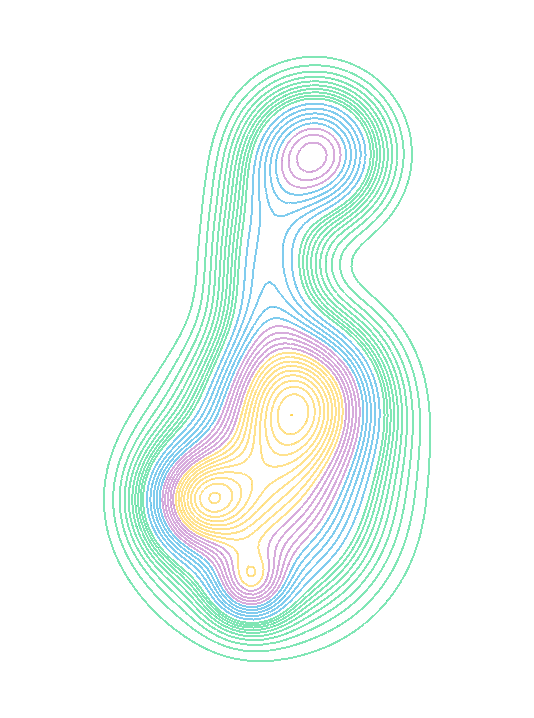
\includegraphics[trim=100 25 75 0, clip, angle=280, scale=0.25]{scripts/figures/scalar_contour.png}
    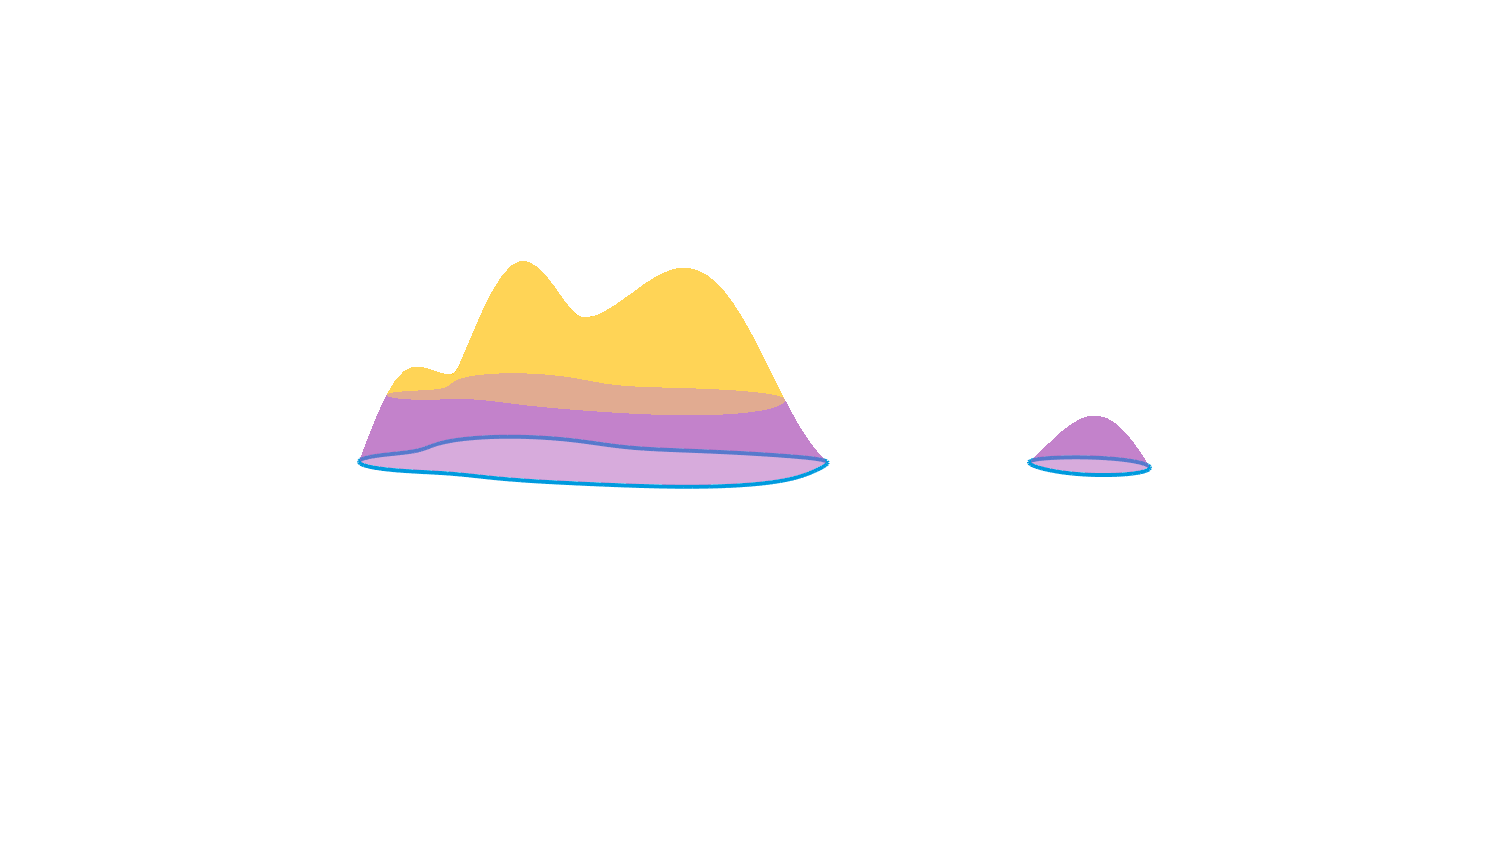
\includegraphics[trim=200 300 200 200, clip, width=0.5\textwidth]{../scripts/figures/surf/ass1_C_side.png}
    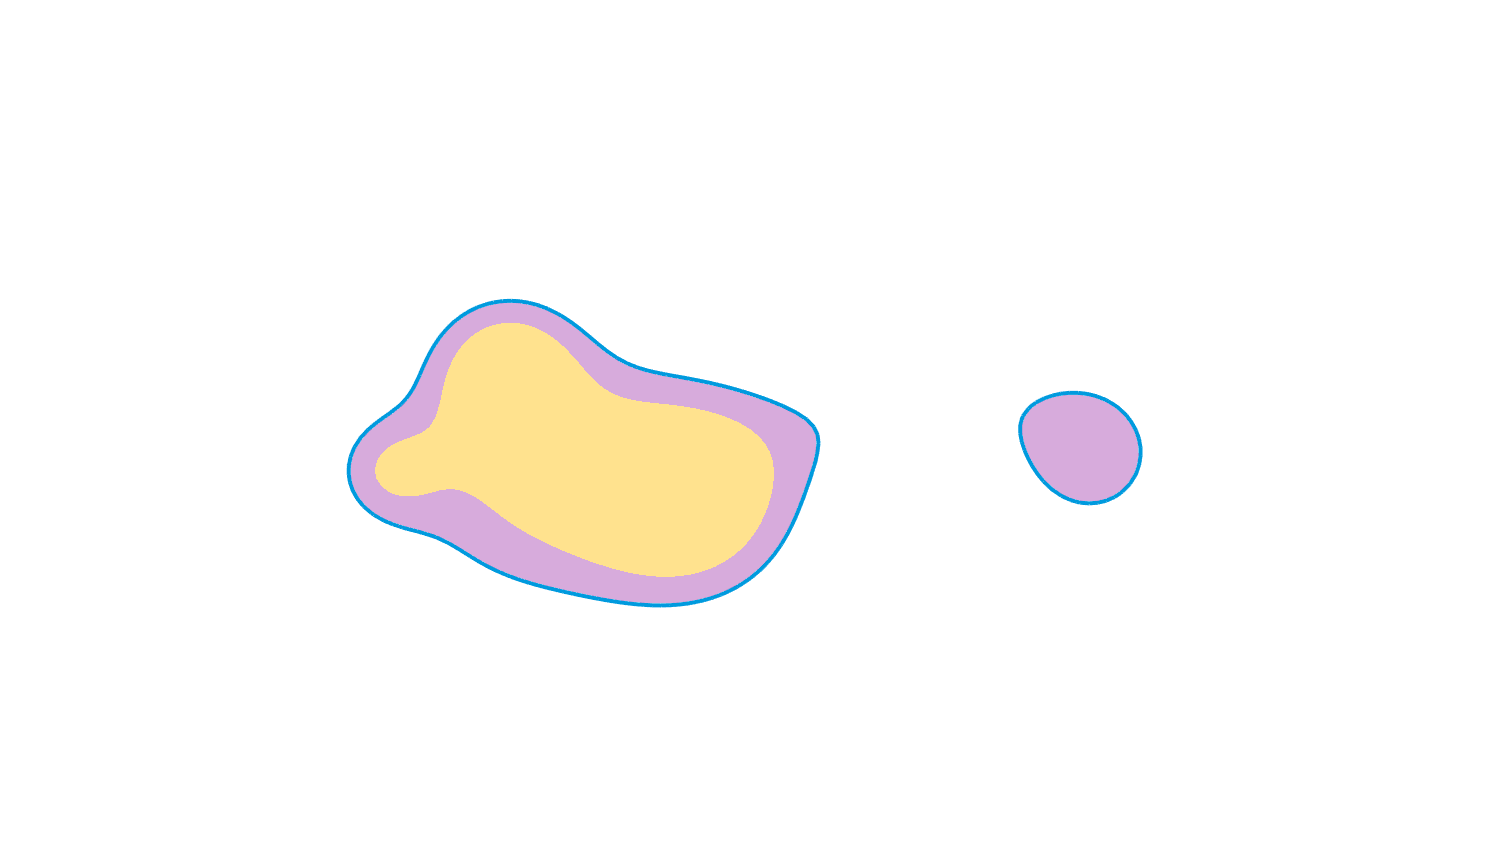
\includegraphics[trim=300 150 200 200, clip, width=0.3\textwidth]{../scripts/figures/surf/ass1_C_top.png}
    
\includegraphics[trim=200 300 200 200, clip, width=0.5\textwidth]{../scripts/figures/surf/ass1_D_side.png}
    
\includegraphics[trim=300 150 200 200, clip, width=0.3\textwidth]{../scripts/figures/surf/ass1_D_top.png}
    % 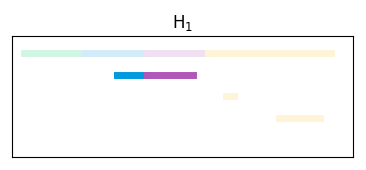
\includegraphics[scale=0.7]{scripts/figures/scalar_barcode_H1-masked.png}
  \end{textblock*}
\end{frame}

\begin{frame}
  \frametitle{{\small Assumption 1 and the Geometric TCC}}

  % \[\begin{tikzcd}
  %   \hom_0(\overline{B_{\omega+c(\delta+\zeta)}},\overline{D})\arrow{d}{m} \arrow{r}{j} &
  %   \hom_0(\overline{B_\omega}, \overline{D}) \arrow{d}{\ell} \\
  %   %
  %   \hom_0(\overline{Q_{\omega+c\delta}^\delta}, \overline{P^\delta}) \arrow{r}{i} &
  %   \hom_0(\overline{Q_{\omega-c\zeta}^\delta}, \overline{P^\delta}).
  % \end{tikzcd}\]

  \begin{theorem}[Geometric TCC]
    % Let $j : \hom_0(\cmp{B_{\omega+c(\delta+\zeta)}},\cmp{D})\to \hom_0(\cmp{\B},\cmp{D})$ and $i : \hom_0(\cmp{\QQ^\of}, \cmp{P^\of})\to \hom_0(\cmp{\Q^\of}, \cmp{P^\of})$ be induced by inclusion.
    %
    If $j$ is surjective and $\mathbf{rk}~i\geq \mathbf{rk}~j$ then $D\setminus B_\omega\subseteq P^\delta$ and $Q_{\omega-c\zeta}^\delta$ surrounds $P^\delta$ in $D$.
  \end{theorem}
\end{frame}

\begin{frame}
  \frametitle{{\small Duality, Assumption 2, and the Algorithmic TCC}}

  % \begin{itemize}
  %   \item Can't compute homology of complements: duality
  %   \item don't know number of connected components: assumption 2
  %   \item Rips-\v Cech interleaving and the Algorithmic TCC
  % \end{itemize}

  \textbf{Duality:} $\hom_d(P^\e,Q_z^\e)\cong\hom_0(D\setminus Q_z^\e, D\setminus P^\e)$.

  % \begin{textblock*}{12cm}(1cm,4.5cm)
  %
  % \end{textblock*}
\end{frame}


\begin{frame}
  \frametitle{{\small Duality, Assumption 2, and the Algorithmic TCC}}

  % \begin{itemize}
  %   \item Can't compute homology of complements: duality
  %   \item don't know number of connected components: assumption 2
  %   \item Rips-\v Cech interleaving and the Algorithmic TCC
  % \end{itemize}

  \only<1>{\begin{textblock*}{11cm}(1cm,2cm)
    \textbf{Assumption 2:} $\hom_0(D\setminus B_\omega\hookrightarrow D\setminus B_{\omega-c(\delta+\zeta)})$ is \emph{injective}.
  \end{textblock*}}

  \begin{textblock*}{12cm}(1cm,4.5cm)
    \includegraphics<1>[trim=200 300 200 200, clip, width=0.5\textwidth]{../scripts/figures/surf/ass2_C_side.png}
    \includegraphics<1>[trim=300 200 200 200, clip, width=0.3\textwidth]{../scripts/figures/surf/ass2_C_top.png}
    \includegraphics<1>[trim=200 300 200 200, clip, width=0.5\textwidth]{../scripts/figures/surf/ass2_B_side.png}
    \includegraphics<1>[trim=300 200 200 200, clip, width=0.3\textwidth]{../scripts/figures/surf/ass2_B_top.png}
  \end{textblock*}

  \only<2>{\begin{lemma}\label{lem:assumption2}
    If $\hom_0(D\setminus B_\omega\hookrightarrow D\setminus B_{\omega+c(\delta+\zeta)})$ is injective and each component of $D\setminus B_\omega$ contains a point in $P$ then $\mathbf{dim}~\hom_0(\rips^\delta(P\setminus Q_{\omega-c\zeta})) \geq \mathbf{dim}~\hom_0(D\setminus B_\omega)$.
  \end{lemma}}
\end{frame}

\begin{frame}
  \frametitle{{\small Duality, Assumption 2, and the Algorithmic TCC}}

  % \begin{itemize}
  %   \item Can't compute homology of complements: duality
  %   \item don't know number of connected components: assumption 2
  %   \item Rips-\v Cech interleaving and the Algorithmic TCC
  % \end{itemize}
  \begin{small}
    \[ \hom_k(\rips^\e(P, Q_w))\xrightarrow{J_w^\e}\hom_k(\cech^\e(P, Q_w))\xrightarrow{I_w^\e}\hom_k(\rips^\e(P, Q_w))\]
    % so
    % \[\mathbf{rk}~\hom_d(\cech^{\delta}(P, Q_{\omega-c\zeta})\hookrightarrow\cech^{\delta}(P, Q_{\omega+c\delta})) \geq\mathbf{rk}~ \hom_d(\rips^{\delta}(P, Q_{\omega-c\zeta})\hookrightarrow\rips^{2\delta}(P, Q_{\omega+c\delta}))\]

    \begin{theorem}[Algorithmic TCC]\label{thm:algo_tcc}
      Suppose $\hom_0(D\setminus B_{\omega+c(\delta+\zeta)}\hookrightarrow D\setminus B_\omega)$ is surjective and $\hom_0(D\setminus B_\omega\hookrightarrow D\setminus B_{\omega-c(\delta+\zeta)})$ is injective.

       If $\mathbf{rk}~\hom_d(\rips^\delta(P, Q_{\omega -c\zeta})\hookrightarrow \rips^{2\delta}(P, Q_{\omega+c\delta})) \geq \mathbf{dim}~\hom_0(\rips^\delta(P\setminus Q_{\omega-c\zeta}))$ then $D\setminus B_\omega\subseteq P^\delta$ and $Q_{\omega-c\zeta}^\delta$ surrounds $P^\delta$ in $D$.
    \end{theorem}
  \end{small}

  % \begin{textblock*}{12cm}(1cm,4.5cm)
  %
  % \end{textblock*}
\end{frame}

% !TeX root = ../main.tex

\paragraph{Algorithms and Cohomology}

From a computational perspective, a great deal of progress has been made to improve the original reduction algorithm in a number of ways.
While the running time of the reduction is cubic in the number of simplices it has been shown that this can be improved to matrix multiplication time using Zigzag persistence~\cite{milosavljevic2011zigzag}.
However, a number of simple modifications improve on this worst-case bound~\cite{chen2011persistent,bauer2014clear} and additional work has been done on computing persistence in parallel~\cite{lewis15parallel} and in a distributed setting~\cite{tahbaz10distributed,bauer2014distributed}.
\emph{The overlap in assumptions made by the TCC and SFA can be used to modify the standard reduction algorithm to efficiently verify coverage during the persistence computation.}

One key observation is that it is often more efficient to compute persistent \emph{cohomology}.
As vector spaces, cohomology is dual to homology, and for reasonable spaces it is known that the persistence barcodes produced by persistent homology and cohomology are the same~\cite{todo}.
% This allows one to compute persistent cohomology instead of persistent homology, and this is often more efficient.
In fact, the reduction algorithm is shown to be the same for persistent homology an cohomology, simply acting in opposite directions~\cite{desilva11duality}.
However, while the barcodes produced are the same, the information captured by homology and cohomology is not.
While homology operates on \emph{cycles} representing \emph{holes} cohomology operates on \emph{cocycles} representing \emph{obstructions}.
Each feature of a barcode is associated with a representative (co)cycle that is often considered a by-product of the persistence computation.
In fact, many recent modifications to the reduction algorithm explicitly abandon these representatives for efficiency~\cite{todo}.
However, these representative encode useful information, and some interesting applications specifically require cocycle representatives~\cite{desilva11circular}.
\emph{Representative (co)cycles can be used to merge the relative persistence diagrams provided by the proposed approach in order to recover the full diagram.}

% !TeX root = ../main.tex

For a pair $(A, B)$ in a topological space $X$ and any $R$ module $G$ let $\hom^k(A, B; G)$ denote the \textbf{singular cohomology} of $(A,B)$ (with coefficients in $G$).
Let $\hom^k_c(A, B; G)$ denote the corresponding \textbf{singular cohomology with compact support}.
For any compact pair $(A,B)$ there is an isomorphism $\hom^k_c(A, B; G)\to\hom^k(A, B; G)$.

Corollary\ref{cor:univ_coef} follows from the Universal Coefficient Theorem for singular homology (and cohomology) as vector spaces over a field $\FF$, as the dual vector space $\Hom(\hom_k(A, B), \FF)$ is isomorphic to $\hom_k(A, B; \FF)$ for any finitely generated $\hom_k(A, B)$.

\begin{corollary}\label{cor:univ_coef}
  For a topological pair $(A, B)$ and a field $\FF$ such that $\hom_k(A, B)$ is finitely generated there is a natural isomorphism
  \[\nu : \hom^k(A, B; \FF)\to \hom_k(A, B; \FF).\]
\end{corollary}

Let $\overline{\hom}^k(A, B; G)$ be the \textbf{Alexander-Spanier cohomology} of the pair $(A,B)$, defined as the limit of the direct system of neighborhoods $(U,V)$ of the pair $(A, B)$.
Let $\overline{\hom}^k_c(A, B; G)$ denote the corresponding \textbf{Alexander-Spanier cohomology with compact support} where $\overline{\hom}^k_c(A, B; G)\cong\overline{\hom}^k(A, B; G)$ for any compact pair $(A, B)$.

\begin{theorem}[\textbf{Alexander-Poincar\'e-Lefschetz Duality} (Spanier~\cite{spanier1989algebraic}, Theorem 6.2.17)]\label{thm:alexander}
  Let $X$ be an orientable $d$-manifold and $(A, B)$ be a compact pair in $X$.
  Then for all $k$ and $R$ modules $G$ there is a (natural) isomorphism
  \[\lambda : \hom_k(X\setminus B, X\setminus A; G)\to \overline{\hom}^{d-k}(A, B; G).\]
\end{theorem}

A space $X$ is said to be \textbf{homologically locally connected in dimension $n$} if for every $x\in X$ and neighborhood $U$ of $x$ there exists a neighborhood $V$ of $x$ in $U$ such that $\tilde{\hom}_n(V)\to\tilde{\hom}_n(U)$ is trivial for $k\leq n$.

\begin{lemma}[Spanier p. 341, Corollary 6.9.6]\label{lem:alexander_iso}
  Let $A$ be a closed subset, homologically locally connected in dimension $n$, of a Hausdorff space $X$, homologically locally connected in dimension $n$.
  If $X$ has the property that every open subset is paracompact, $\mu : \overline{\hom}_c^k(X,A; G)\to \hom_c^k(X, A; G)$ is an isomorphism for $k\leq n$ and a monomorphism for $q = n+1$.
\end{lemma}

In the following we will assume homology (and cohomology) over a field $\FF$.

\begin{lemma}\label{cor:alexander_iso}
  Let $X$ be an orientable $d$-manifold and $(A,B)$ a compact pair of locally path connected subspaces in $X$.
  Then
  \[\xi : \hom_d(X\setminus B, X\setminus  A)\to \hom_0(A, B)\]
  is a natural isomorphism.
\end{lemma}
\begin{proof}
  Because $X$ is orientable and $(A,B)$ are compact $\lambda : \hom_d(X\setminus B, X\setminus A)\to \overline{\hom}^{0}(A, B)$ is an isomorphism by Theorem~\ref{thm:alexander}.
  Note that
  Moreover, because every subset of $X$ is (hereditarily) paracompact every open set in $A$, with the subspace topology, is paracompact.
  For any neighborhood $U$ of a point $x$ in a locally path connected space there must exist some neighborhood $V\subset U$ of $x$ that is path connected in the subspace topology.
  As $\tilde{\hom}_0(V) = 0$ for any nonempty, path connected topological space $V$ (see Spanier p. 175, Lemma 4.4.7) it follows that $A$ (resp. $B$) are homologically locally connected in dimension $0$.
  Because $(A,B)$ is a compact pair the singular and Alexander-spanier cohomology modules of $(A,B)$ with compact support are isomorphic to those without, thus $\mu:\overline{\hom}^{0}(A, B)\to \hom^0(A, B)$ is an isomorphism.
  By Corollary~\ref{cor:univ_coef} we have a natural isomorphism $\nu : \hom^0(A, B)\to\hom_0(A, B)$ thus the composition $\xi := \nu\circ\mu\circ\lambda : \hom_d(X\setminus B, X\setminus  A)\to \hom_0(A, B)$ is a natural isomorphism.
\end{proof}

\begin{lemma}\label{lem:duality_apply}
  Let $\X$ be an orientable $d$-manifold let $D$ be a compact subset of $\X$.
  Let $P$ be a finite subset of $D$ such that $P^\e\subset \intr_\X(D)$ and $Q\subseteq P$.

  If $D\setminus Q^\e$ and $D\setminus P^\e$ are locally path connected then there is a natural isomorphism
  \[ \xi : \hom_d(P^\e,Q^\e)\to \hom_0(D\setminus Q^\e, D\setminus P^\e).\]
\end{lemma}
\begin{proof}
  Because $Q^\e$ and $P^\e$ are open in $D$ and $D$ is compact in $\X$ the complement $D\setminus Q^\e$ is closed in $D$, and therefore compact in $\X$.
  Moreover, because $P^\e\subset \intr_\X(D)$, $\hom_d(\X\setminus(D\setminus P^\e), \X\setminus(D\setminus Q^\e)) = \hom_d(P^\e, Q^\e)$.
  As we have assumed these complements are locally path connected by assumption we have a natural isomorphism $\xi : \hom_d(P^\e, Q^\e)\to \hom_0(D\setminus Q^\e, D\setminus P^\e)$
  by Lemma~\ref{cor:alexander_iso}.
  %
  % Because $\e > \varrho_D$ the covers by metric balls associated with $P^\e$ and $Q^\e$ are good, so we have isomorphisms $\N : \hom_d(\cech^\e(P, Q))\to \hom_d(P^\e, Q^\e)$ for all $Q\subseteq P$ by the Nerve Theorem.
  % So the composition $\xi\N := \xi\circ\N$ is an isomorphism.
  % Moreover, because $\xi$ is natural and $\N$ commutes with maps induced by inclusions by the persistent nerve lemma the composition $\xi\N$ does as well.
\end{proof}

% \begin{lemma}\label{lem:duality_apply}
%   Let $\X$ be an orientable $d$-manifold let $D$ be a compact subset of $\X$ with strong convexity radius $\varrho_D > \e$.
%   Let $P$ be a finite subset of $D$ such that $P^\e\subset \intr_\X(D)$ and $Q\subseteq P$.
%
%   If $D\setminus Q^\e$ and $D\setminus P^\e$ are locally path connected then there is an isomorphism
%   \[ \xi\N : \hom_d(\cech^\e(P,Q))\to \hom_0(D\setminus Q^\e, D\setminus P^\e)\]
%   that commutes with maps induced by inclusions.
% \end{lemma}
% \begin{proof}
%   Because $Q^\e$ and $P^\e$ are open in $D$ and $D$ is compact in $\X$ the complement $D\setminus Q^\e$ is closed in $D$, and therefore compact in $\X$.
%   Moreover, because $P^\e\subset \intr_\X(D)$, $\hom_d(\X\setminus(D\setminus P^\e), \X\setminus(D\setminus Q^\e)) = \hom_d(P^\e, Q^\e)$.
%   As we have assumed these complements are locally path connected by assumption we have a natural isomorphism $\xi : \hom_d(P^\e, Q^\e)\to \hom_0(D\setminus Q^\e, D\setminus P^\e)$
%   by Lemma~\ref{cor:alexander_iso}.
%
%   Because $\e > \varrho_D$ the covers by metric balls associated with $P^\e$ and $Q^\e$ are good, so we have isomorphisms $\N : \hom_d(\cech^\e(P, Q))\to \hom_d(P^\e, Q^\e)$ for all $Q\subseteq P$ by the Nerve Theorem.
%   So the composition $\xi\N := \xi\circ\N$ is an isomorphism.
%   Moreover, because $\xi$ is natural and $\N$ commutes with maps induced by inclusions by the persistent nerve lemma the composition $\xi\N$ does as well.
% \end{proof}

% The requirement that our complements are locally path connected is necessary in order to satisfy the general statement of the duality theorem.
% A rigorous investigation of the minimal assumptions that can be made on $\X$ and $D$ is beyond the scope of this paper.
% We note that, in practice, it likely suffices to assume that there exists a triangulation of $P^\e$ that is a subcomplex of some refinement of a triangulation of $\X$ (see~\cite{cavanna2017when},~\cite{julian83alexander}).


% % \begin{theorem}[\textbf{Alexander-Poincar\'e Duality} (Julian et. al.~\cite{julian83alexander}, Theorem 5.1)]\label{thm:alexander}
% %   Let $K$ be an abstract simplicial complex that is a combinatorial oriented $d$-manifold.
% %   Let $L$ be a subcomplex of some refinement of $K$ and $M$ be a subcomplex of $L$.
% %   Let $\overline{L}$ and $\overline{M}$ denote the complements of $L$ and $M$ as subcomplexes of $K$ that do not share vertices with the original complexes.
% %   Then for all $k$ there is a natural isomorphism
% %   \[ \hom^k(L, M)\to \hom_{d-k}(\overline{M},\overline{L}). \]
% % \end{theorem}
%
% % \begin{corollary}
% %   Let $X$ be a topological space and $D$ be a compact subspace of $X$.
% %   Let $(U, V)$ be a topological pair of spaces in $D$ and suppose there exists a triangulation $\Delta X$ of $X$ such that there exists triangulation $\Delta U$ of $U\subset$ that is a subcomplex of some refinement of $\Delta X$ and a triangulation $\Delta V$ of $V$ that is a subcomplex of $\Delta U$.
% %   Then for all $k$ there is a natural isomorphism
% %   \[ \hom^k(U, V)\to\hom_{d-k}(D\setminus U, D\setminus V).\]
% % \end{corollary}
%
%
% \begin{corollary}\label{cor:univ_coef}
%   Let $(A, B)$ be a topological pair and $\FF$ be a field such that $\hom_k(A, B; \FF)$ is finitely generated.
%   Then there is a natural isomorphism
%   \[\hom^k(A, B; \FF)\to \hom_k(A, B; \FF).\]
% \end{corollary}
% \begin{proof}
%   As $\mathrm{Ext}(\Hom(A, B), \FF) = 0$ for any field $\FF$ the map
%   \[\hom^k(A, B; \FF)\to \Hom(\hom_k(A, B), \FF)\]
%   in the natural short exact sequence provided by Theorem~\ref{thm:univ_coef} is a natural isomorphism.
%   The result follows from the fact that $\hom_k(A, B; \FF)$ is finitely generated, and is therefore isomorphic to the dual vector space $\Hom(\hom_k(A, B), \FF)$.
% \end{proof}
%
% % \begin{theorem}[\textbf{Universal Coefficient Theorem} (Munkres p. 337, Corollary 56.4)]\label{thm:univ_coef}
% %   Let $(A,B)$ be a topological pair such that $\hom_k(A, B)$ is finitely generated for all $k$.
% %   Then for all $k$ and any abelian group $G$ there is a natural exact sequence
% %   \[ 0\to\mathrm{Ext}(\hom^{k+1}(A, B), G)\to \hom_k(A, B; G)\to \Hom(\hom^k(A, B), G)\to 0.\]
% %   This sequence splits, but not naturally.
% % \end{theorem}
%
% \begin{theorem}
%   Let $X$ be a topological space and $D$ be a compact subspace of $X$.
%   Suppose there exists a triangulation $\Delta X$ of $X$ that is a combinatorial oriented $d$-manifold.
%   Let $(U, V)$ be a topological pair of spaces in $D$ and $\FF$ be a field such that $\hom_k(U,V;\FF)$ is finitely generated for all $k$.
%
%   If there exists a pair of triangulations $(\Delta U, \Delta V)$ of the pair $(U, V)$ such that $\Delta U$ is a subcomplex of some refinement of $\Delta X$ then there is a natural isomorphism
%   \[ \hom_d(U, V; \FF)\to \hom_0(X\setminus V, X\setminus U; \FF).\]
% \end{theorem}
% \begin{proof}
%   By Theorem~\ref{thm:alexander} we have a natural isomorphism
%   \[ \hom^d(\Delta U, \Delta V; \FF)\to \hom_{0}(\overline{\Delta V}, \overline{\Delta U}; \FF) \]
%   where $\overline{\Delta V}$ and $\overline{\Delta U}$ denote the complements of $\Delta V$ and $\Delta U$ as subcomplexes of $\Delta X$ that do not share vertices with their respective original complexes.
%   \textbf{TODO}\footnote{$\hom^d(U, V;\FF)\cong \hom^d(\Delta U, \Delta V;\FF),\ \hom_{0}(\overline{\Delta V}, \overline{\Delta U}; \FF) \cong \hom_0(X\setminus V, X\setminus U; \FF).$}
%
%   Because $\hom_d(U, V; \FF)$ is finitely generated $\hom_d(U, V;\FF)\cong\hom^d(U, V; \FF)$ by Corollary~\ref{cor:univ_coef}.
%   It follows that the composition
%   \[\hom_d(U, V; \FF)\to \hom^d(U,V;\FF)\to\hom_0(X\setminus V, X\setminus U; \FF)\]
%   is a natural isomorphism as desired.
% \end{proof}
% % \begin{proof}
% %   \begin{itemize}
% %     \item By Theorem~\ref{thm:univ_coef} we have a short exact sequence
% %       \[ 0\to\mathrm{Ext}(\hom^{d+1}(\Delta U, \Delta V), G)\to \hom_d(\Delta U, \Delta V; G)\to \Hom(\hom^d(\Delta U, \Delta V), G)\to 0\]
% %       for any abelian group $G$.
% %       Because $\Delta U,\Delta V$ are subcomplexes of the combinatorial $d$-manifold $\Delta X$, $\hom^{d+1}(\Delta U, \Delta V) = 0$, so $\hom_d(\Delta U, \Delta V; G)\to \Hom(\hom^d(\Delta U, \Delta V), G)$ is an isomorphism.
% %     \item By Theorem~\ref{thm:alexander} we have a natural isomorphism $\hom^d(\Delta U, \Delta V)\to \hom_0(\overline{\Delta V},\overline{\Delta U})$.
% %       Therefore, because we have natural\footnote{\textbf{TODO} natural short exact $\implies$ natural isomorphism.} isomorphisms $\hom_d(\Delta U, \Delta V; G)\to \Hom(\hom^d(\Delta U, \Delta V), G)$ for all abelian groups $G$, we have a natural isomorphism (\textbf{TODO} prove it).
% %       \[\hom_d(\Delta U, \Delta V)\to \hom_0(\overline{\Delta V},\overline{\Delta U}).\]
% %     \item Because $\hom_d(U, V)\cong \hom_d(\Delta U, \Delta V)$ and $\hom_0(X\setminus V, X\setminus U)\cong \hom_0(\overline{\Delta V},\overline{\Delta U})$ (\textbf{TODO} prove it\footnote{$(X\setminus V, X\setminus U)$ or $(D\setminus V, D\setminus U)$?}), we have a natural isomorphism
% %     \[ \hom_d(U, V)\to \hom_0(X\setminus V, X\setminus U). \]
% %   \end{itemize}
% % \end{proof}
%
%
% %
% % \begin{theorem}[\textbf{Alexander Duality} (Spanier p. 296, Theorem 6.2.17)]
% %   Let $U$ be an orientation over $R$ of an $d$-manifold $X$ and let $(A, B)$ be a compact pair in $X$.
% %   Then for all $k$ and $R$ modules $G$ there is a natural isomorphism
% %   \[ \hom_k(X\setminus B, X\setminus A; G)\to\overline{\hom}^{d-k}(A, B; G).\]
% % \end{theorem}
% %
% % \begin{lemma}
% %   Let $U$ be an orientation over $R$ of an $d$-manifold $X$ and let $(A, B)$ be a compact pair in $X$ such that $\hom_k(A, B)$ is finitely generated for all $k$.
% %   Then for all $R$ modules $G$ there is a natural isomorphism
% %   \[ \hom_0(X\setminus B, X\setminus A; G)\to\hom_d(A, B; G). \]
% % \end{lemma}
% % \begin{proof}
% %   \textbf{TODO}
% % \end{proof}


% \paragraph{Problem Statement}
% % !TeX root = ../main.tex

The TCC works by checking the number of generators in the top-dimensional relative homology of a domain modulo its boundary.
For reasonable spaces this number is known to be equal to the number of connected components of the domain.
One can therefore confirm that a sample covers the domain by checking that the number of generators in the top-dimensional relative homology of the sample, modulo ``sampled boundary,'' is equal to the number of connected components of the underlying space.
It is important to note that this test not only covers the domain, but also that we have a sub-sample of points close to the boundary.
We refer to this as having a sample that is \emph{topologically representative} of the underlying bounded domain.

In its original form the TCC is stated as a criteria for coverage by a sensor network in a coordinate free setting---coordinates of sensors are not provided, only some limited connectivity information.
Without coordinates there is no way to determine which points are close to the boundary.
The points making up the sampled boundary must therefore be labelled manually.
This requirement is perhaps the main reason why the TCC can so rarely be applied in practice.

It can be shown that this assumption can be removed by requiring that our input points sample some unknown $c$-Lipschitz function.
This requirement is natural for applications to data analysis, where data represents local measurements of some underlying process.
Given a threshold on function values that can be used to define a bounding subset of the domain we can define our sampled boundary by their function values alone.
Moreover, the TCC requires additional \emph{regularity assumptions} that are required in order to establish the minimum resolution of the sample.
Traditionally, these assumptions required information about the geometry of the domain, and were made in terms of the \emph{smoothness} of its boundary.
Now, these assumptions can be stated directly in terms of the persistent homology of the function itself.

From this perspective, computing the TCC and approximating the persistent homology of a scalar field overlap in a number of ways.
In fact, the coverage condition can be extracted directly from the persistence diagram, and the quality of the approximation depends coverage.
It is in this way that one can verify that a persistence diagram is representative of the scalar field by leveraging topological priors similar to those required by the TCC.
Not only is the criterion encoded in this diagram, but its computation produces a \emph{fundamental class} for the domain that can be used to compute topological duals.



% \paragraph{Objectives}
% % !TeX root = ../main.tex

I propose adapting the TCC as a way to provide verified scalar field analysis.
% This is to develop a theoretical foundation for how topological methods can be used to \emph{verify} data with respect to prior information about the topology of the underlying space.
This work will re-cast the TCC as a way to check that a sample is \emph{topologically representative} of the underlying space with assumptions that are more natural to samples of functions.
I will also show how a generalization of these assumptions can be used to prove stability results of the resulting persistence diagram.
This gives a bound on the quality of the approximation that is proportional to the resolution of the sample.
It will also extend existing work on SFA to instances of \emph{partial coverage}.
The goal is to provide a theorem that unifies the assumptions made by the TCC and SFA to assert when that the quality of the diagram approximated by an arbitrary sample can be determined by the diagram itself.

Additional work is motivated by an application involving Lipschitz extensions that requires computing \emph{topological duals} within the persistence computation.
This will extend the existing theory of persistent (co)homology to support duality via the cap product with a fundamental class.
How this can be used with the observation that the TCC provides this fundamental class is currently an open research question.
This work also leads to a new characterization of \emph{pair groups} in persistent (co)homology in terms of long exact sequences.
The theory can then be applied to modify the standard reduction algorithm for persistent (co)homology to pair (co)cycles with dual (co)boundaries.

%
%
\paragraph{Prior Work and Potential Issues}
% !TeX root = ../main_socg.tex

We have extended the Topological Coverage Criterion to the setting of Topological Scalar Field Analysis.
By defining the boundary in terms of a sublevel set of a scalar field we provide an interpretation of the TCC that applies more naturally to data coverage.
We then showed how the assumptions and machinery of the TCC can be used to approximate the persistent homology of the scalar field relative to a static sublevel set.
This relative persistent homology is shown to be related to a truncation of that of the scalar field as whole, and therefore provides a way to approximate a part of its persistence diagram in the presence of un-verified data.

There are a number of unanswered questions and directions for future work.
Our theoretical results were limited by our understanding of duality.
Importantly, a more rigorous treatment of duality allow us to formally link the regularity assumptions made in the TCC and our interleaving
This would allow us to merge the assumptions made in these two statements as our main theorem.
It would also simplify some of the assumptions made on our sample in the statement of the TCC.
Moreover, as duality plays a central role in the TCC it is natural to investigate its role in the analysis of scalar fields.
Our hope is to be able to provide a rigorous comparison between the relative approach and the persistent homology of the superlevel set filtration, leading to connections with Extended Persistence~\cite{cohen09extending}.
% This would not only allow us to apply duality to persistent homology~\cite{desilva11duality}, but also allow us to provide a rigorous comparison between the relative approach and the persistent homology of the superlevel set filtration and explore connections with Extended Persistence~\cite{cohen09extending}.

From a computational perspective, we are particularly interested in the matching problem discussed in Section~\ref{sec:experiments} that can be used to recover the full diagram.
Our statements in terms of sublevel sets can also be generalized to disjoint unions of sub and superlevel sets, where coverage is confirmed in an \emph{interlevel} set.
This, along with a better understanding of the duality between sub and superlevel sets could lead to an iterative approach in which the persistent homology of a scalar field is constructed as data becomes available.
% We also note that computing the diagram of a nested pair of relative Rips complexes that vary in both function values and scale is nontrivial.
% We are interested in finding efficient ways to compute these image diagrams.
% We are also interested in finding efficient ways to compute the image persistent (relative) homology that vary in both scalar and scale.

% The problem of relaxing our assumptions on the boundary can be approached from both a theoretical and computational perspective.
% Ways to avoid the isomorphism we require could be investigated in theory, and the interaction of relative persistent homology and the Persistent Nerve Lemma may be used tighten our assumptions.
% We would also like to conduct a more rigorous investigation on the effect of these assumptions in practice.


\bibliographystyle{unsrt}
\bibliography{bibliography}

% \appendix

\end{document}
